\documentclass[a4paper, 11pt]{article}
\usepackage{comment}
\usepackage{fullpage}
\usepackage{amsmath}
\usepackage{amssymb}
\usepackage{mathtools}
\usepackage{fontspec}
\defaultfontfeatures{Ligatures=TeX}
\usepackage{xfrac}
\usepackage{icomma}
\usepackage[section,below]{placeins}
\usepackage[labelfont=bf,font=small,width=0.9\textwidth]{caption}
\usepackage{subcaption}
\usepackage{graphicx}
\usepackage{grffile}
\usepackage{float}
\floatplacement{figure}{htbp}
\floatplacement{table}{htbp}
\usepackage{booktabs}
\usepackage{hyperref}
\usepackage[ngerman]{babel}
\usepackage{pdfpages}
\begin{document}
\noindent
%\centerline{\small{\textsc{Technische Universität Dortmund}}} \\
\large{\textbf{4. Übungsblatt zur Vorlesung \hfill WS 2017/2018 \\
Statistische Methoden der Datenanalyse \hfill Prof. W. Rhode}} \\
Annika Burkowitz, Sebastian Bange, Alexander Harnisch \\
\noindent\makebox[\linewidth]{\rule{\textwidth}{0.4pt}}

\section*{Aufgabe 12}
\subsection*{a)}
Die untenstehenden Rechnungen zeigen, dass die Population $P_1$ ebenfalls eine
2D Normalverteilung mit den Parametern
\begin{align*}
  \mu_\text{y}^{'} &= a + b\mu_\text{x}=3,1\,, \\
  \sigma_\text{y}^{'} &= \sqrt{\sigma_\text{y|x}^2+b^2\sigma_\text{x}^2}
    = \frac{\sqrt{541}}{10} \approx 2,326\, \text{und}\\
  \rho &= b \frac{\sigma_\text{x}}{\sigma_\text{y}} \approx 0,90286
\end{align*}
beschreibt.

\subsection*{b)}
Beide Populationen werden in einem zweidimensionalen Scatter-Plot dargestellt.
Dazu werden Gaußverteilungen mit $10000$ Werten pro Population und den Parametern
\begin{align*}
  P_0:\;\; &\mu_\text{x} = 0,\;\; \mu_\text{x} = 3,\;\; \sigma_\text{x}=3.5,\;\;
   \sigma_\text{y}=2.6 \quad \text{und} \quad \rho=0.9 \\
  P_1:\;\; &\mu_\text{x} = 6,\;\; \mu_\text{x} = 3.1,\;\; \sigma_\text{x}=3.5,\;\;
  \sigma_\text{y}= \frac{\sqrt{541}}{10} \quad \text{und} \quad \rho\approx 0.90286
\end{align*}
erzeugt und gemeinsam in Abbildung \ref{fig:populationen} dargestellt.
\begin{figure}[H]
  \centering
  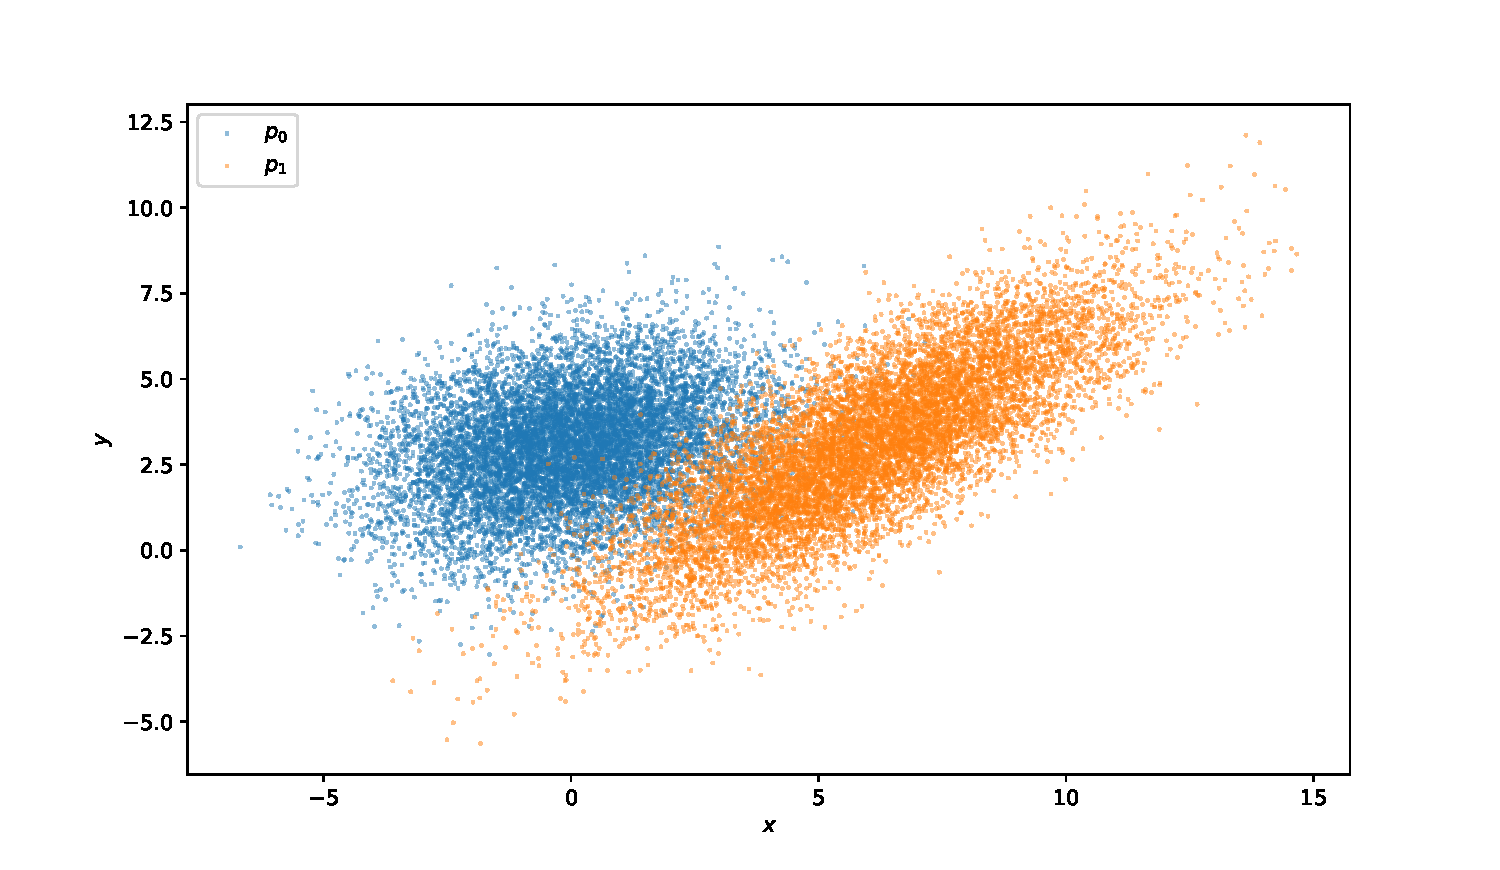
\includegraphics[width=\textwidth]{../A12/A12b.pdf}
  \caption{Zweidimensionaler Scatter-Plot für die Populationen $P_0$ und $P_1$.}
  \label{fig:populationen}
\end{figure}

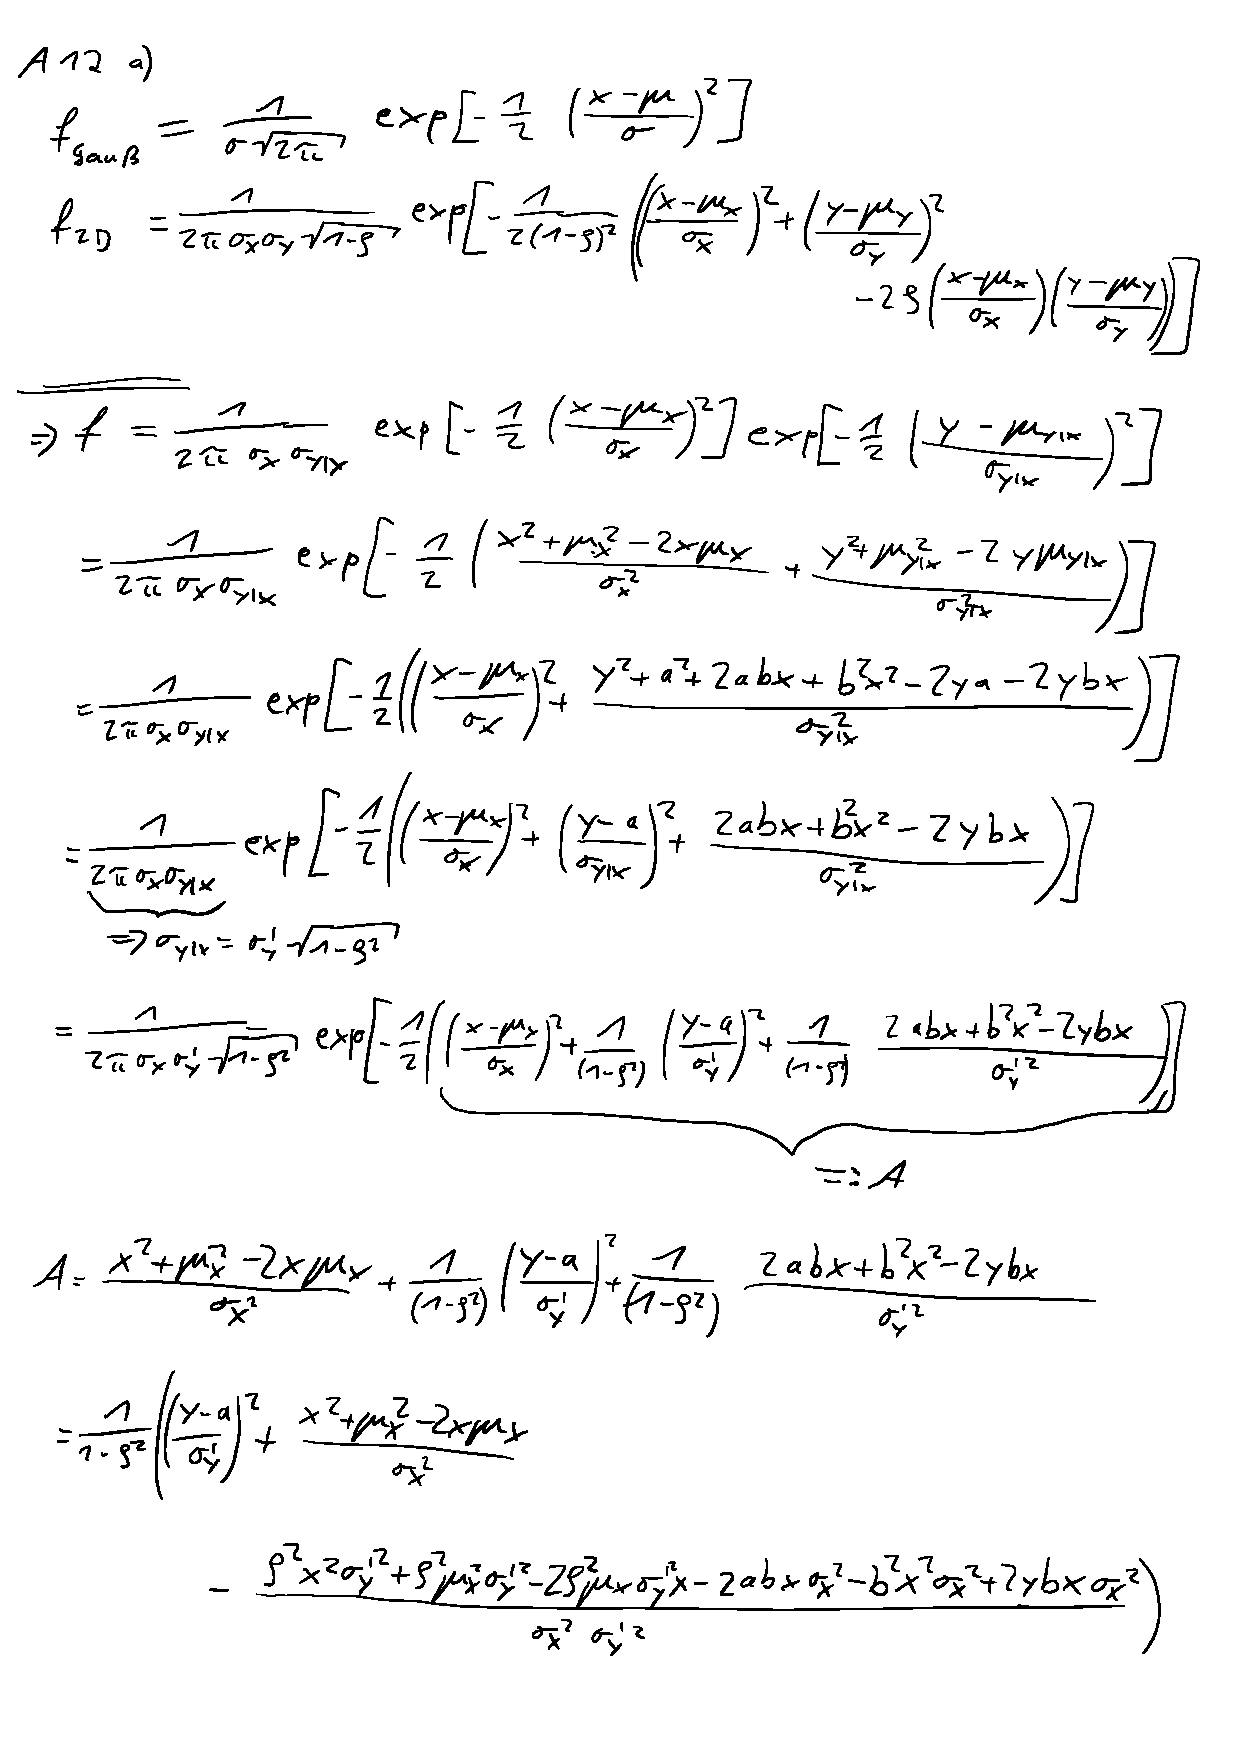
\includepdf[pages=1-3]{../Rechnungen}

\FloatBarrier

\section*{Aufgabe 13}
\subsection*{a)}
Mit den in Aufgabe 12 erzeugten Datenpunkten für die Populationen $P_0$ und $P_1$,
die in einem HDF-File gespeichert wurden, wird erneut ein zweidimensionaler
Scatter-Plot erstellt, in den zusätzlich die Projektionsgeraden
\begin{align*}
  g_1(x)&=0 \\
  g_2(x)&=-\frac{3}{4}x\\
  g_3(x)&=-\frac{5}{4}x
\end{align*}
eingezeichnet werden. Der Plot ist in Abbildung \ref{fig:populationen+geraden}
dargestellt.
\begin{figure}
  \centering
  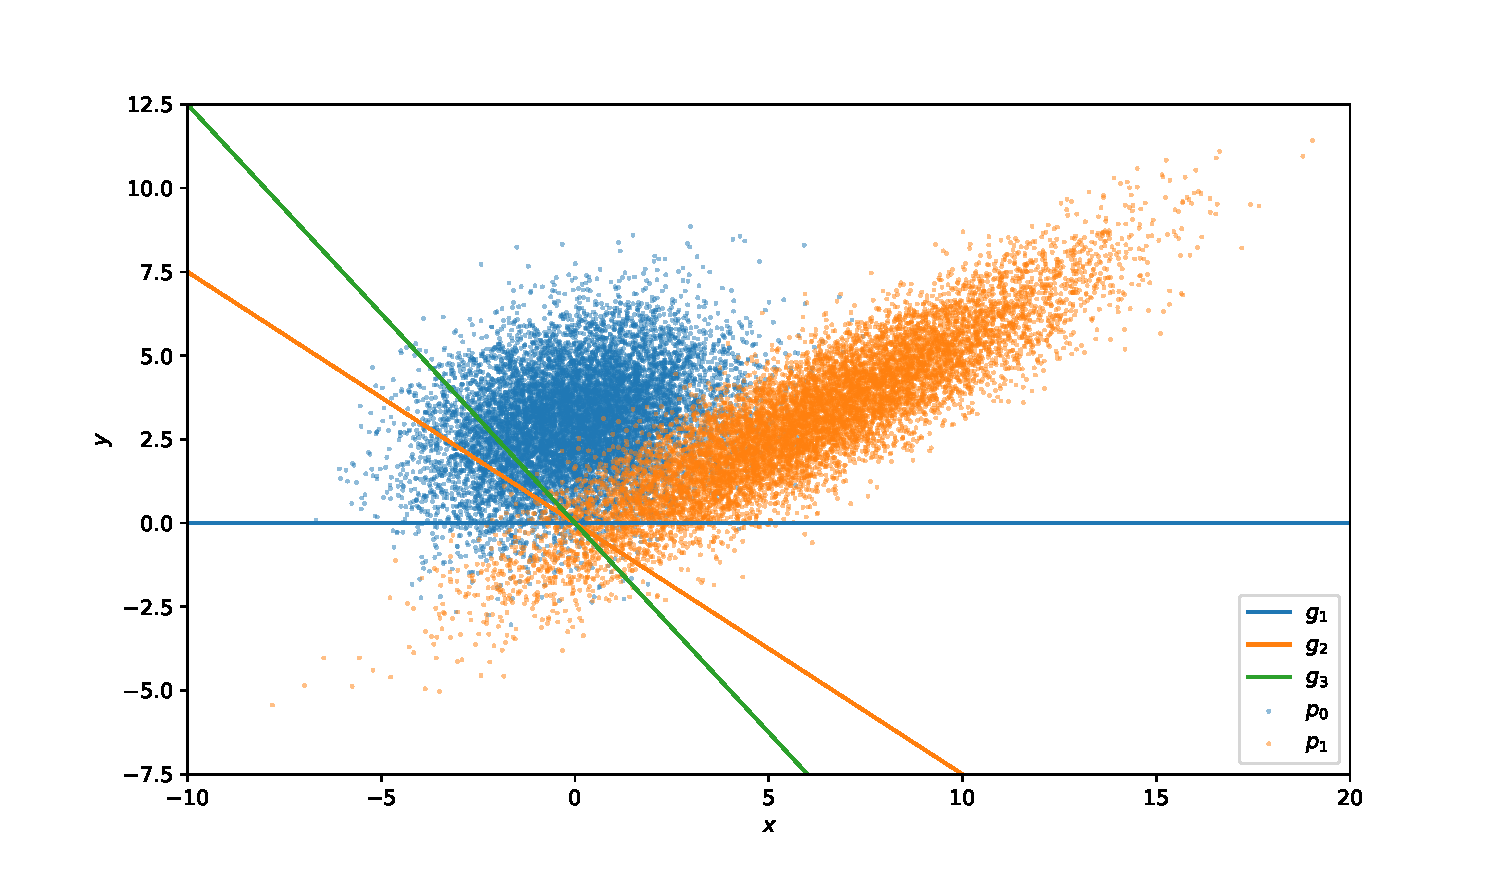
\includegraphics[width=\textwidth]{../A13/A13a_scatter}
  \caption{Zweidimensionaler Scatter-Plot für die Populationen $P_0$ und $P_1$
  und die drei Projektionsgeraden.}
  \label{fig:populationen+geraden}
\end{figure}
\FloatBarrier

\subsection*{b)}
Zunächst werden die normierten Projektionsvektoren für die drei Geraden bestimmt.
Die Projektionsvektoren können dabei direkt aus der Steigung der Geraden abgelesen
werden. Das Vorzeichen wird jeweils so gewählt, dass $P_0$ nach der Projektion
rechts von $P_1$ liegt.
\includepdf[pages=4]{../Rechnungen}
Für die Projektion wird für jeden Datenpunkt $\vec{x_\text{i}}$ das Skalarprodukt
mit den Projektionsvektoren $\vec{p_\text{j}}$ gebildet:
\begin{equation}
  x_\text{i,j,projeziert} = \vec{x_\text{i}} \cdot \vec{p_\text{j}}\,.
\end{equation}
Die projezierten Datenpunkte sind für jeden Projektionsvektor getrennt in den
Histogrammen in Abbildung \ref{fig:hist1}, \ref{fig:hist2} und \ref{fig:hist3}
dargestellt.
\begin{figure}
  \centering
  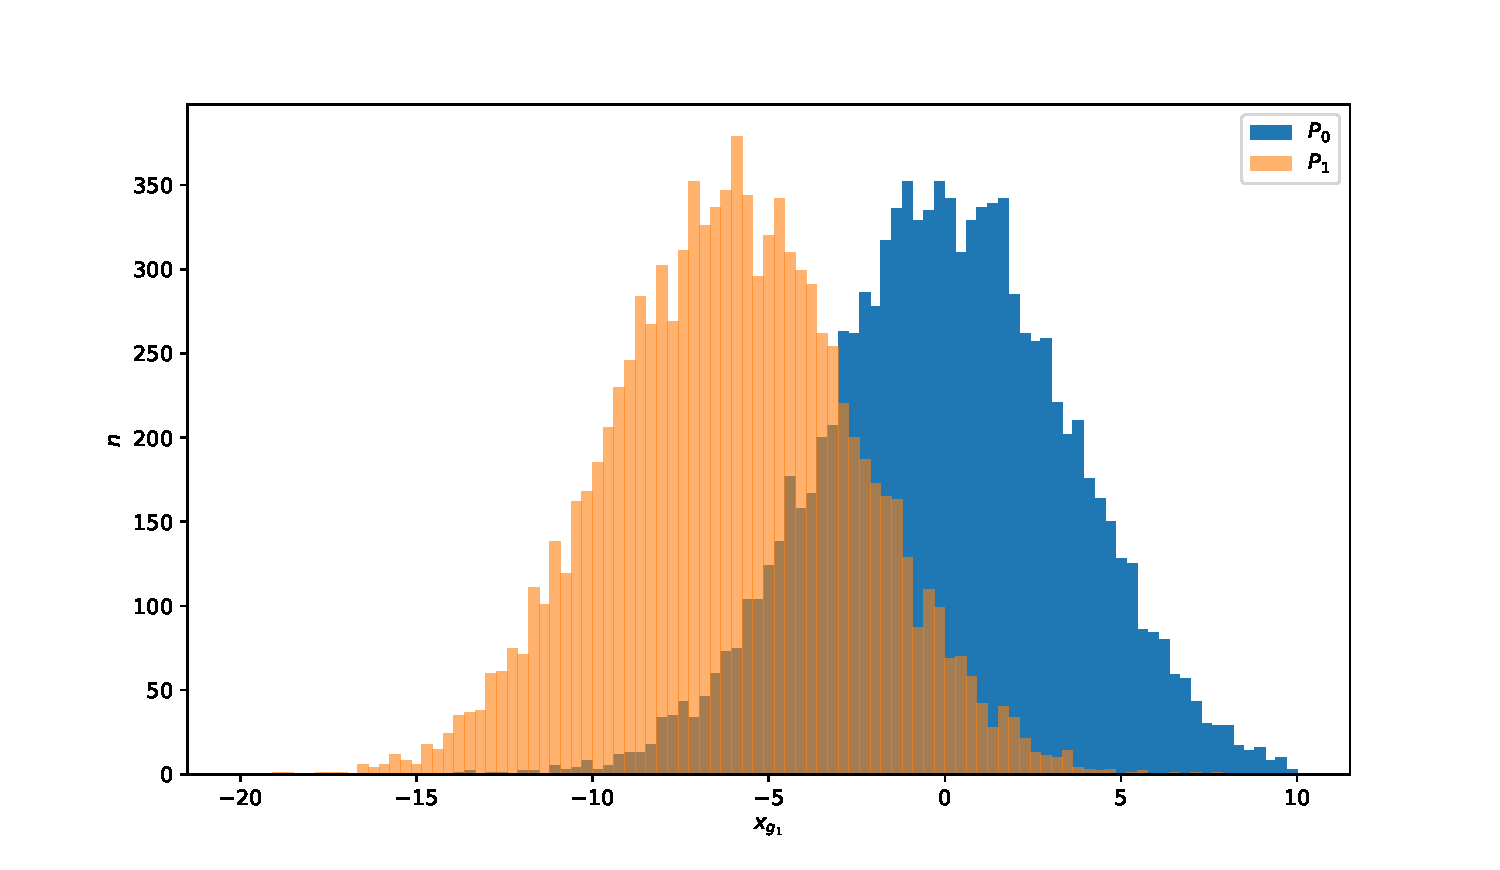
\includegraphics[width=\textwidth]{../A13/A13b_1}
  \caption{Histogramm für die Projektion der Populationen $P_0$ und $P_1$ auf
  die Gerade $g_1$.}
  \label{fig:hist1}
\end{figure}
\begin{figure}
  \centering
  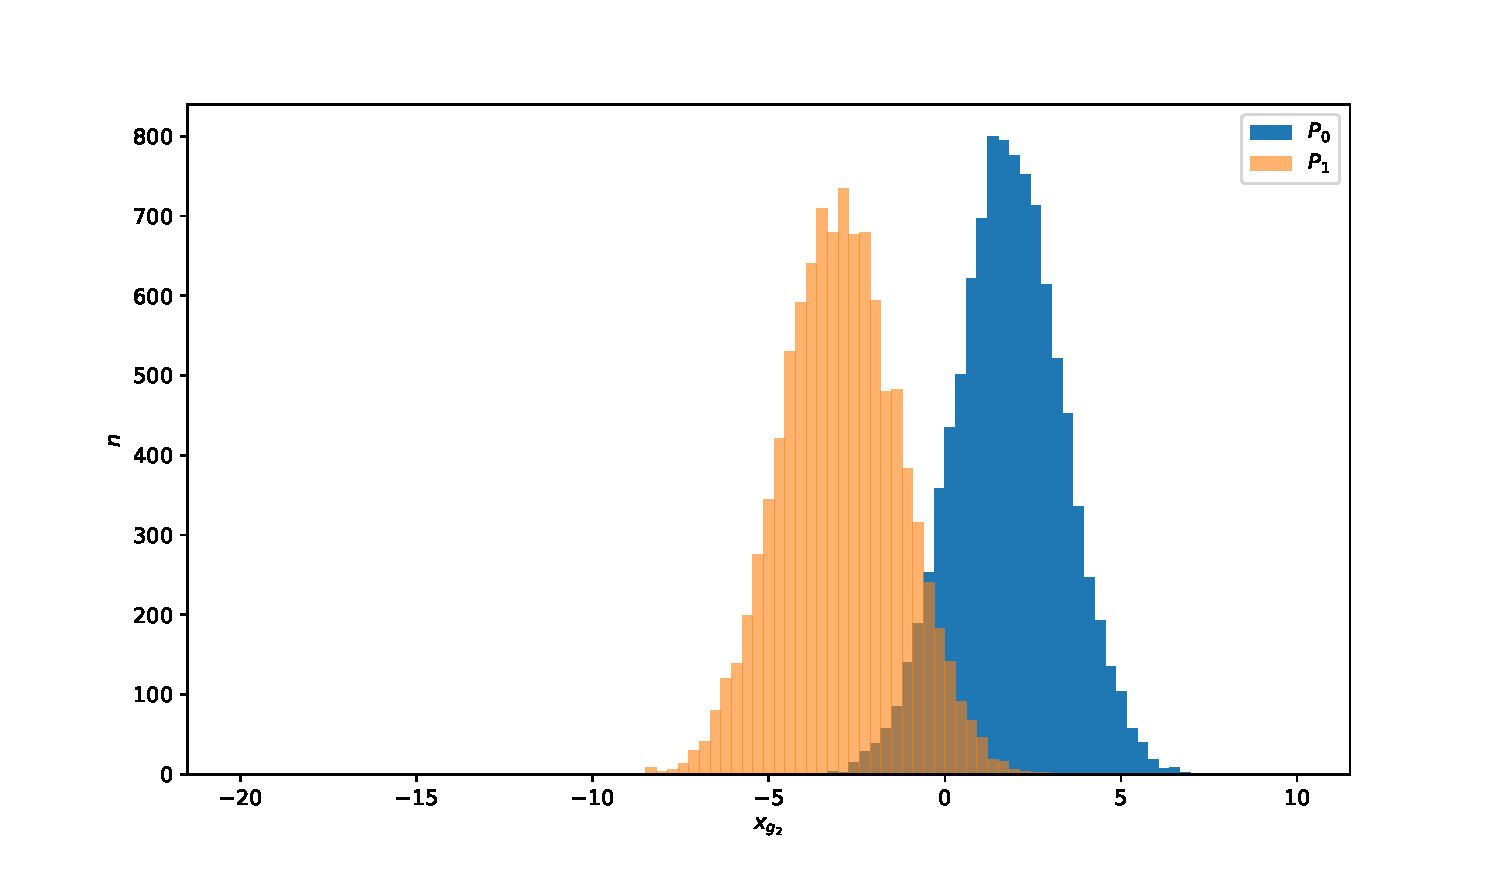
\includegraphics[width=\textwidth]{../A13/A13b_2}
  \caption{Histogramm für die Projektion der Populationen $P_0$ und $P_1$ auf
  die Gerade $g_2$.}
  \label{fig:hist2}
\end{figure}
\begin{figure}
  \centering
  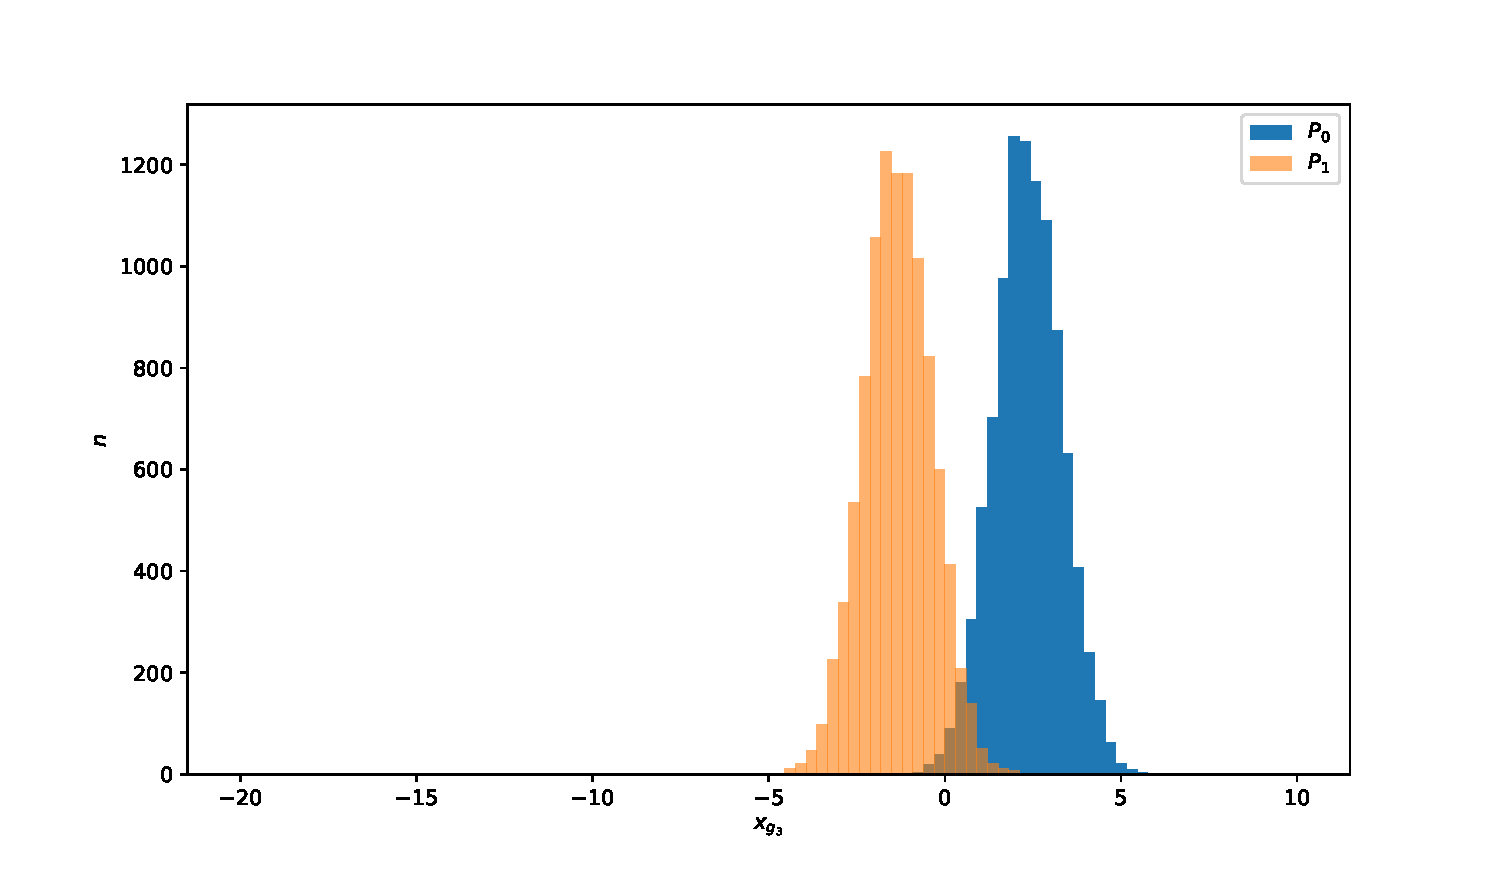
\includegraphics[width=\textwidth]{../A13/A13b_3}
  \caption{Histogramm für die Projektion der Populationen $P_0$ und $P_1$ auf
  die Gerade $g_3$.}
  \label{fig:hist3}
\end{figure}
\FloatBarrier

\subsection*{c)}
Die Population $P_0$ wird als Signal betrachtet, $P_1$ stellt den Untergrund dar.
Abhängig vom gewählten Schnitt $\lambda_\text{cut}$ wird für jede Projektion die
Effizienz, die Reinheit und die Genauigkeit bestimmt. Dazu werden die projezierten
Datenpunkte sortiert und die Anzahl der true positiv (tp), false negative (fn),
der true negative (tn) und der false positive (fp) wird abhängig vom Schnitt
gezählt.
\begin{align*}
  \text{Effizienz } &= \frac{\text{tp}}{\text{tp + fp}} \\
  \text{Reinheit } &= \frac{\text{tp}}{\text{tp + fn}} \\
  \text{Genauigkeit } &= \frac{\text{tp + tn}}{\text{tp + tn + fp + fn}}
\end{align*}
Die Effizienz, Reinheit und Genauigkeit sind für jede der drei Projektionen
in den Abbildungen \ref{fig:effrein1}, \ref{fig:effrein2} und \ref{fig:effrein3}
dargestellt.
\begin{figure}[H]
  \centering
  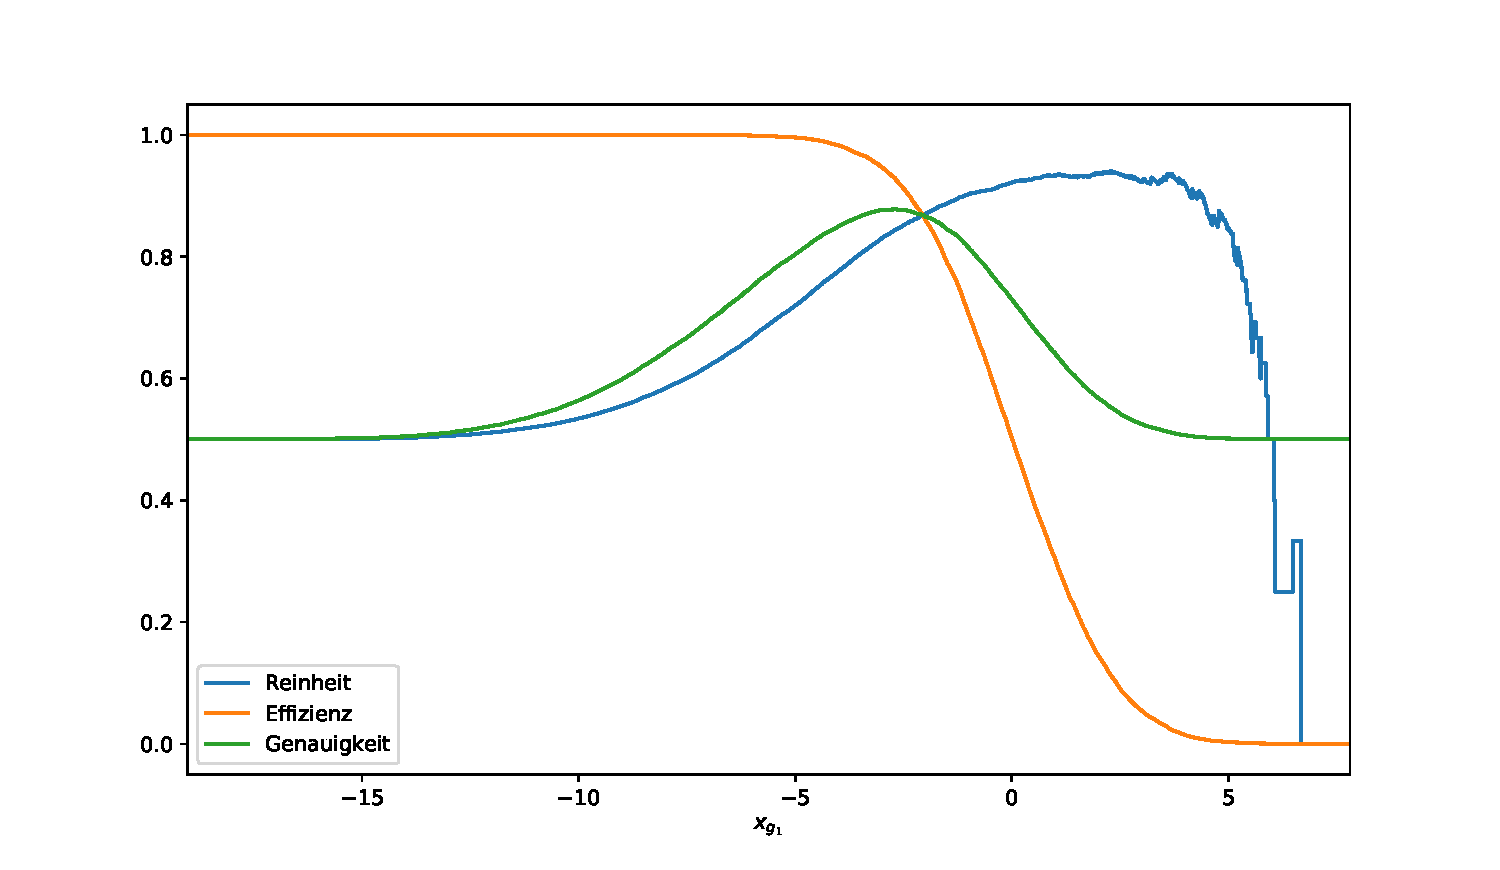
\includegraphics[width=\textwidth]{../A13/A13c_0}
  \caption{Effizenz, Reinheit und Genauigkeit in Abhängigkeit von $\lambda_\text{cut}$
   für die Projektion der Populationen $P_0$ und $P_1$ auf die Gerade $g_1$.}
  \label{fig:effrein1}
\end{figure}
\begin{figure}[H]
  \centering
  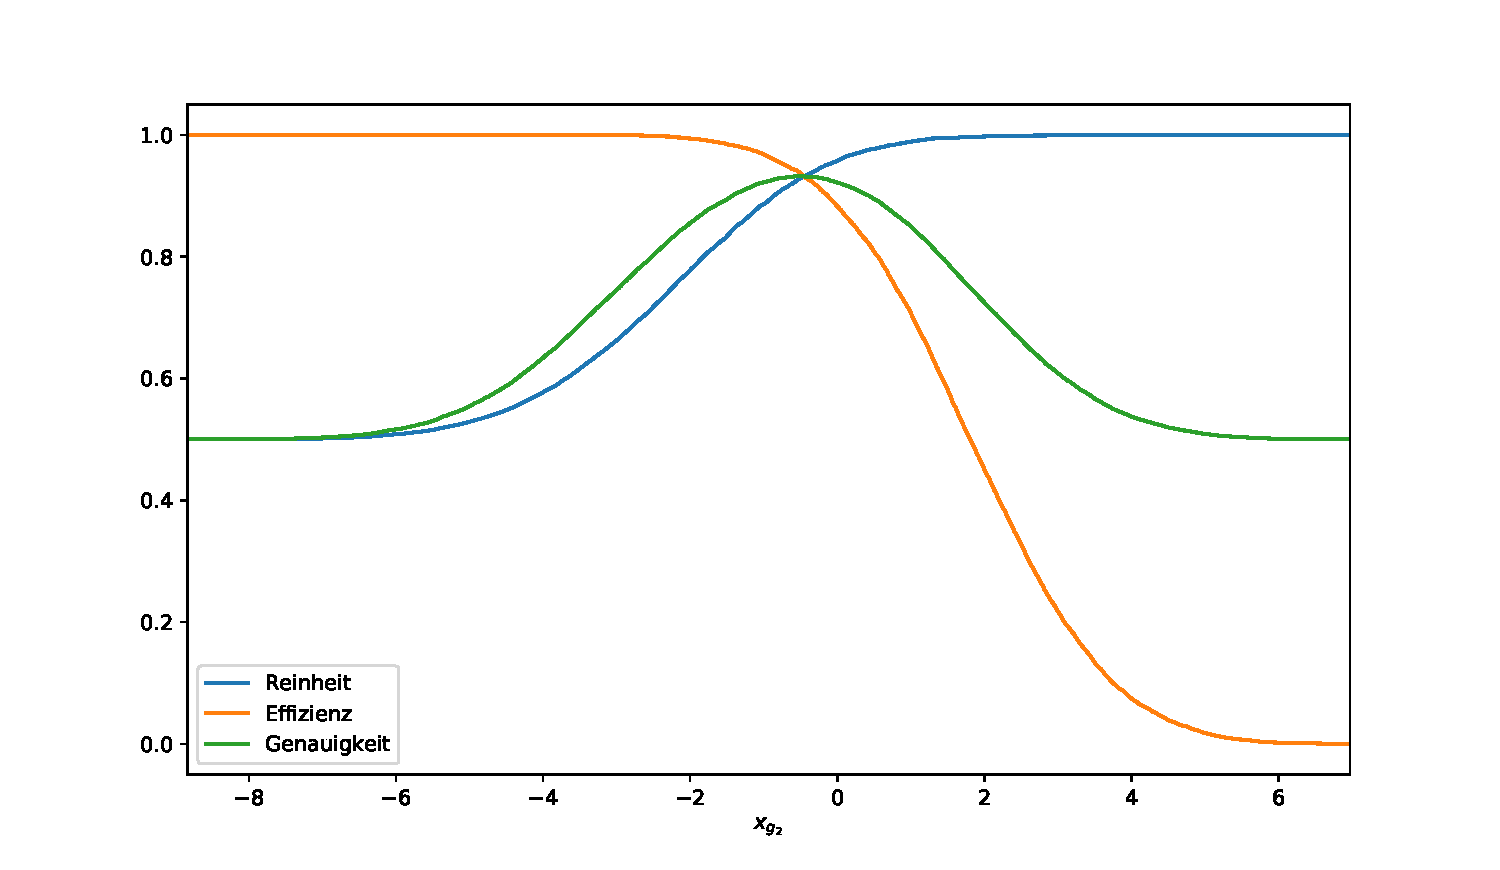
\includegraphics[width=\textwidth]{../A13/A13c_1}
  \caption{Effizenz, Reinheit und Genauigkeit in Abhängigkeit von $\lambda_\text{cut}$
   für die Projektion der Populationen $P_0$ und $P_1$ auf die Gerade $g_2$.}
  \label{fig:effrein2}
\end{figure}
\begin{figure}[H]
  \centering
  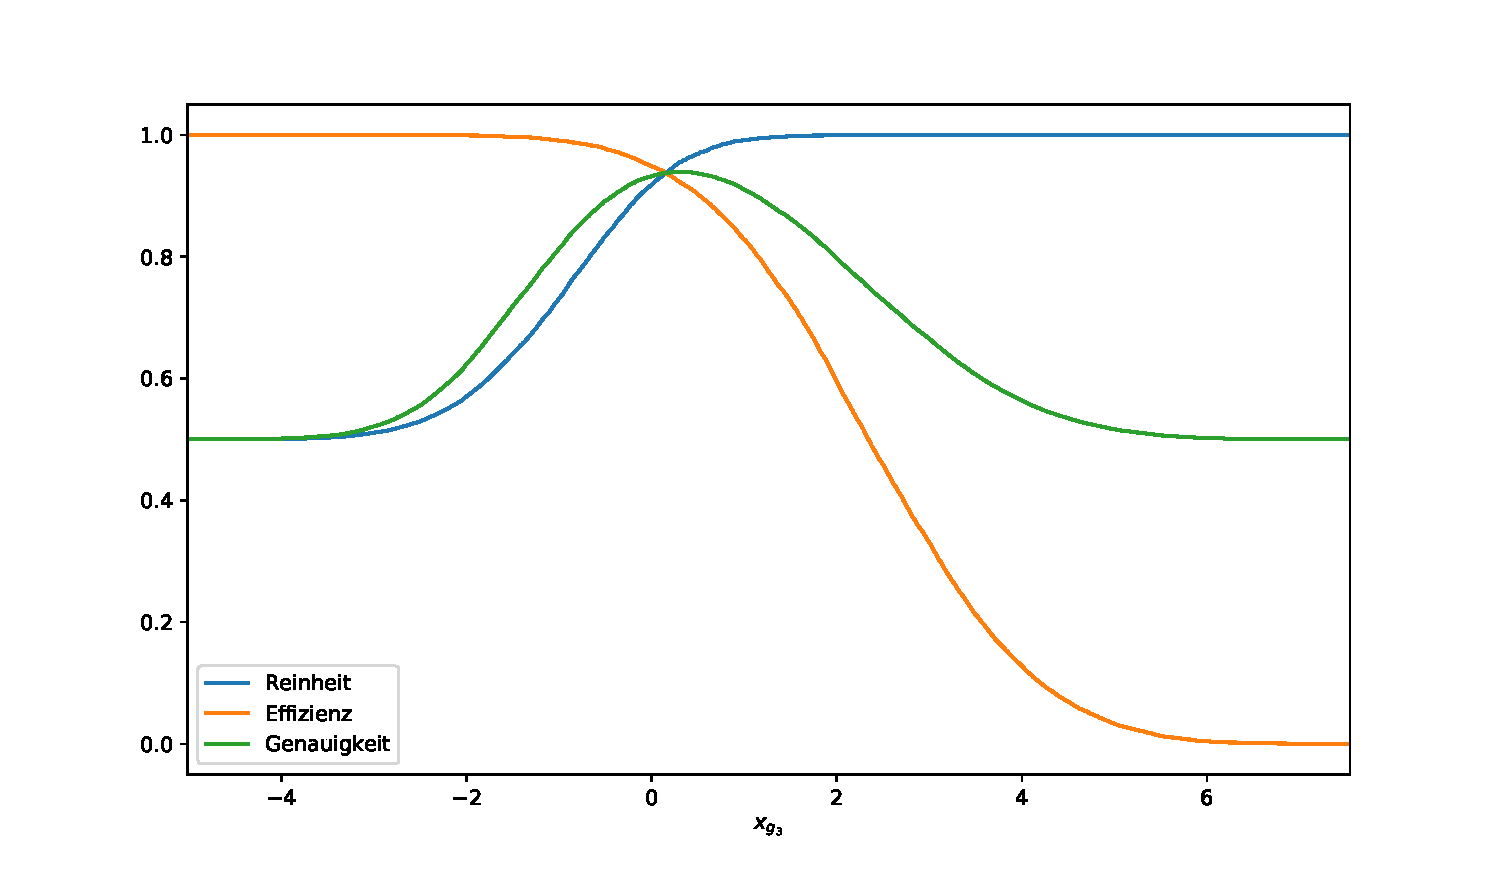
\includegraphics[width=\textwidth]{../A13/A13c_2}
  \caption{Effizenz, Reinheit und Genauigkeit in Abhängigkeit von $\lambda_\text{cut}$
   für die Projektion der Populationen $P_0$ und $P_1$ auf die Gerade $g_3$.}
  \label{fig:effrein3}
\end{figure}

\FloatBarrier
%\section*{Aufgabe 14}
\includepdf[pages=5-11]{../Rechnungen}

\FloatBarrier
\section*{Aufgabe 15}
\subsection*{a) \normalfont{Siehe unten.}}

\subsection*{b) \normalfont{Siehe Code.}}

\subsection*{c)}
Die mit dem Metropolis-Algorithmus erzeugten Zufallszahlen werden in Abbildung
\ref{fig:metropolis-hist} als Histogramm dargestellt und mit einer Gaußverteilung
mit $\mu = -3$ und $\sigma=2$ verglichen. Es zeigt sich eine gute Übereinstimmung.
Auffällig ist, dass rechts vom Mittelwert der Verteilung deutlich häufiger
Zahlen mit einer sehr geringen Wahrscheinlichkeitsdichte gezogen werden, als
links vom Mittelwert. Dies liegt an dem gewählten Startwert $x_0=15$ und der
Anlaufphase des Algorithmus (vgl. d)).
\begin{figure}
  \centering
  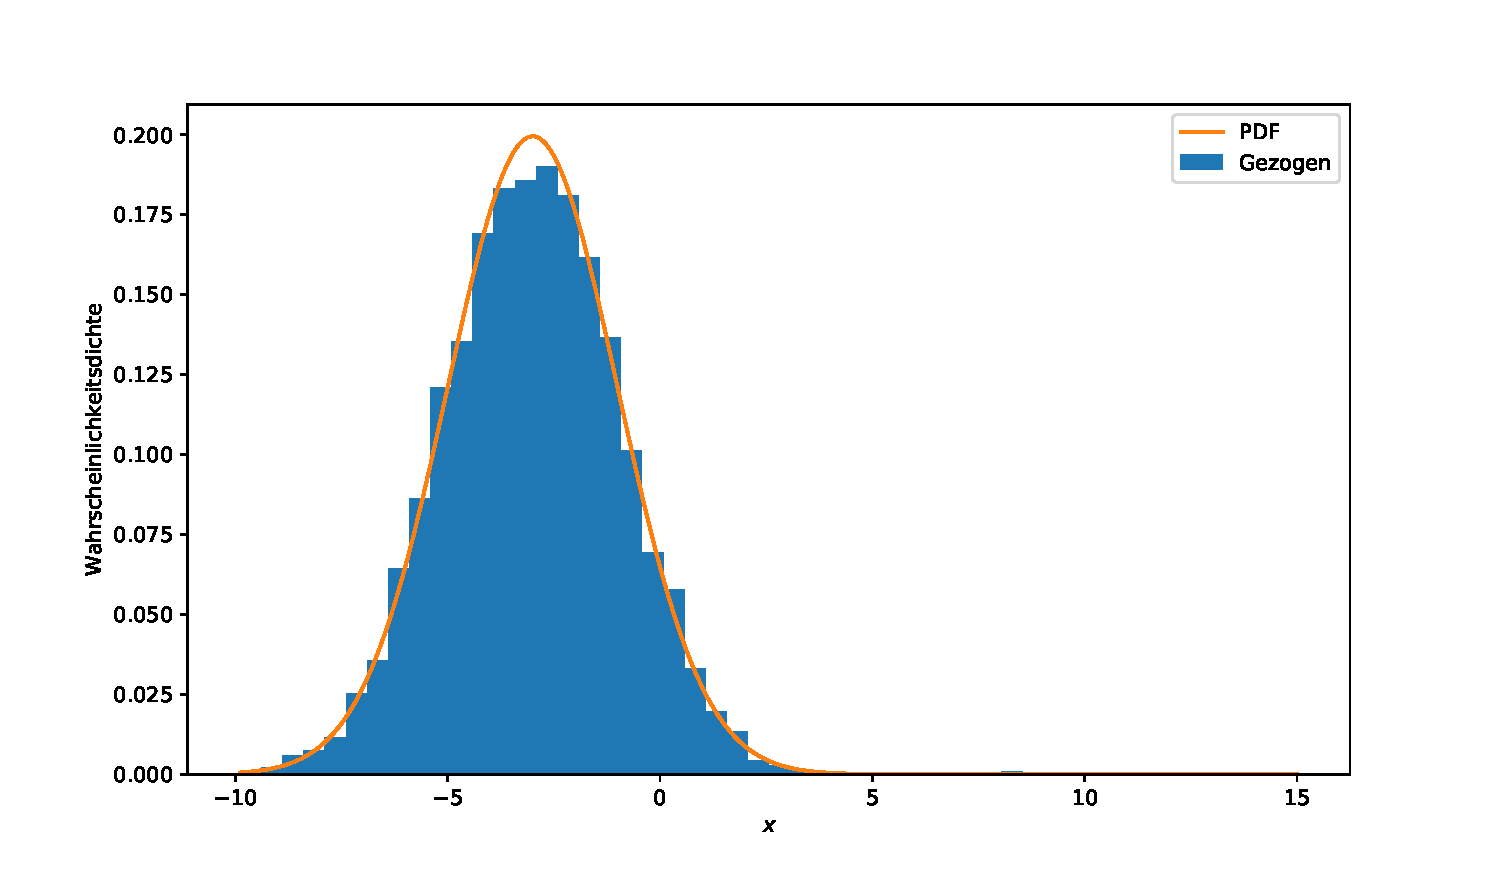
\includegraphics[width=\textwidth]{../A15/A15c}
  \caption{Histogramm von 10000 mit dem Metropolis-Algorithmus erzeugten
  Zufallszahlen ($x_0=15$, stepsize $=2$, $\mu = -3$ und $\sigma=2$) und Vergleich
  mit der analytischen Form der Gaußverteilung.}
  \label{fig:metropolis-hist}
\end{figure}
\FloatBarrier

\subsection*{d)}
Die erzeugten Zufallszahlen werden gegen die Iteration, in der sie erzeugt wurden,
aufgetragen. Der sogenannte Trace-Plot ist in Abbildung \ref{fig:trace} dargestellt.
In Abbildung \ref{fig:trace-zoom} ist der Ausschnitt, der die Anlaufphase enthält,
vergrößert dargestellt. In dem Ausschnitt ist deutlich zu erkennen, dass der
Algorithmus mit dem gewählten Startparameter von $x_0 = 15$ etwa 50 Iterationen
benötigt, um in die Nähe des Mittelwerts zu gelangen (Anlaufphase). Daher sollten
die Zufallszahlen, die während der Anlaufphase erzeugt wurden, verworfen werden.
Da 10000 Zufallszahlen gezogen wurden, ist es gut möglich, die ersten 500 Iterationen
zu verwerfen, um einen gewissen Sicherheitsabstand (Faktor 10) zur Anlaufphase
sicherzustellen.
\begin{figure}
  \centering
  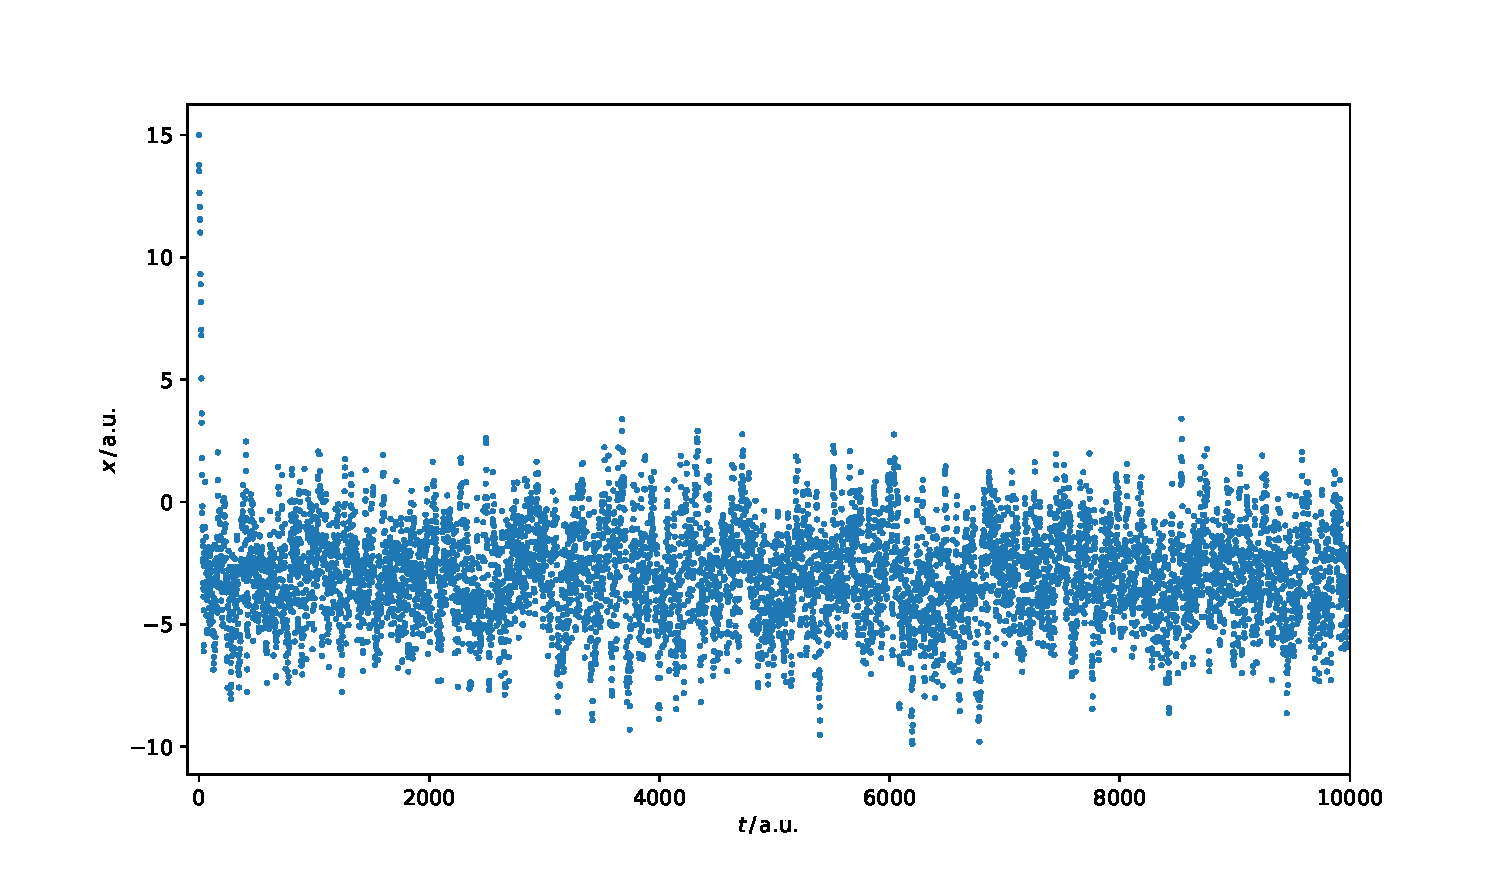
\includegraphics[width=\textwidth]{../A15/A15d}
  \caption{Trace-Plot für die erzeugten Zufallszahlen.}
  \label{fig:trace}
\end{figure}
\begin{figure}
  \centering
  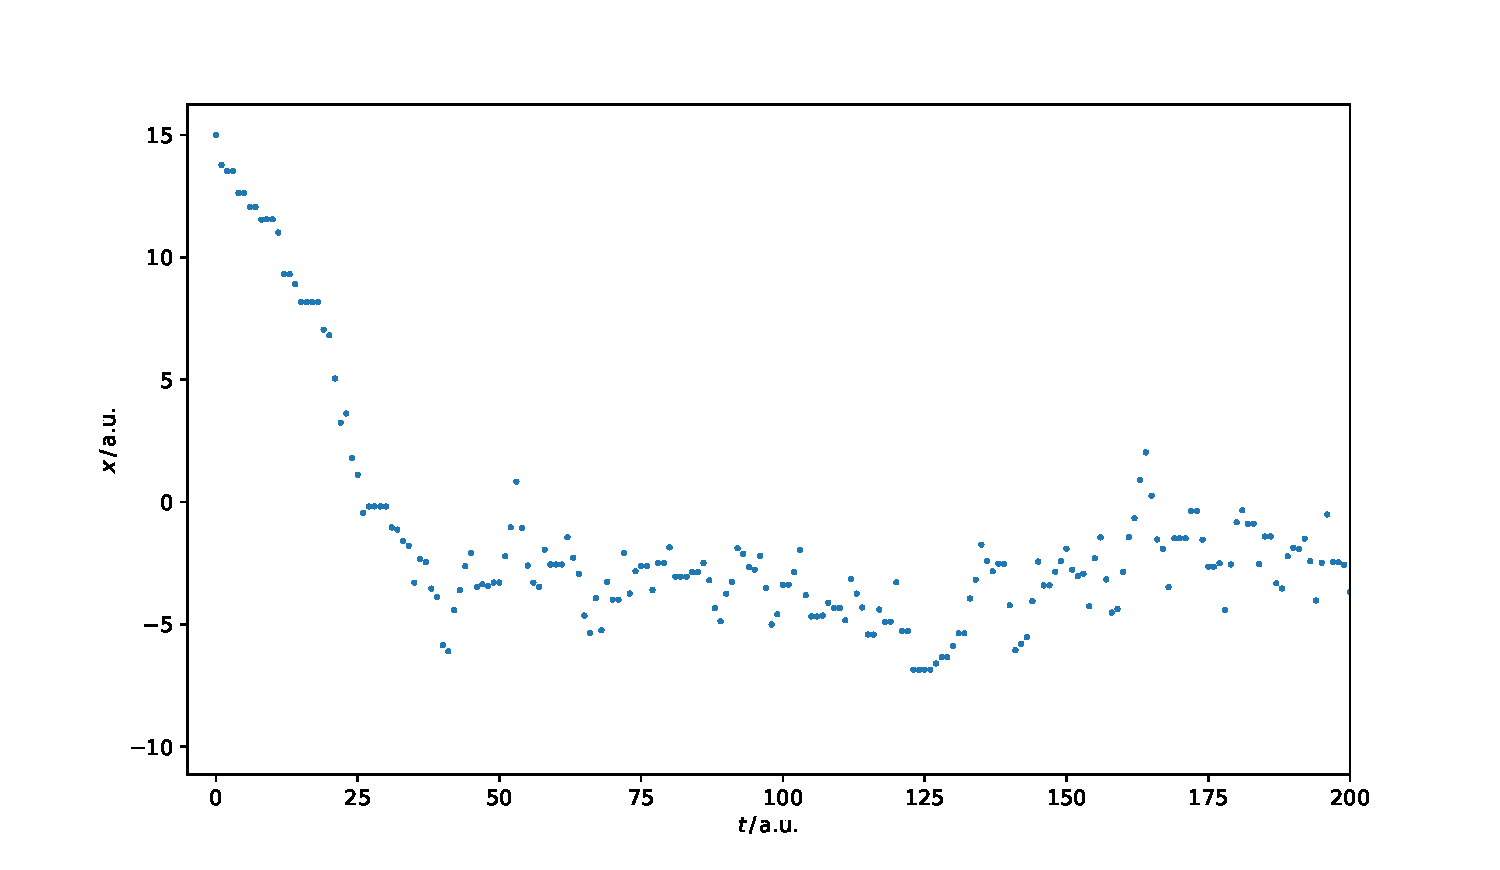
\includegraphics[width=\textwidth]{../A15/A15d_zoom}
  \caption{Trace-Plot (Ausschnitt der Anlaufphase).}
  \label{fig:trace-zoom}
\end{figure}
\FloatBarrier
\includepdf[pages=12]{../Rechnungen}
\end{document}
